% Options for packages loaded elsewhere
\PassOptionsToPackage{unicode}{hyperref}
\PassOptionsToPackage{hyphens}{url}
\PassOptionsToPackage{dvipsnames,svgnames,x11names}{xcolor}
%
\documentclass[
]{agujournal2019}

\usepackage{amsmath,amssymb}
\usepackage{iftex}
\ifPDFTeX
  \usepackage[T1]{fontenc}
  \usepackage[utf8]{inputenc}
  \usepackage{textcomp} % provide euro and other symbols
\else % if luatex or xetex
  \usepackage{unicode-math}
  \defaultfontfeatures{Scale=MatchLowercase}
  \defaultfontfeatures[\rmfamily]{Ligatures=TeX,Scale=1}
\fi
\usepackage{lmodern}
\ifPDFTeX\else  
    % xetex/luatex font selection
\fi
% Use upquote if available, for straight quotes in verbatim environments
\IfFileExists{upquote.sty}{\usepackage{upquote}}{}
\IfFileExists{microtype.sty}{% use microtype if available
  \usepackage[]{microtype}
  \UseMicrotypeSet[protrusion]{basicmath} % disable protrusion for tt fonts
}{}
\makeatletter
\@ifundefined{KOMAClassName}{% if non-KOMA class
  \IfFileExists{parskip.sty}{%
    \usepackage{parskip}
  }{% else
    \setlength{\parindent}{0pt}
    \setlength{\parskip}{6pt plus 2pt minus 1pt}}
}{% if KOMA class
  \KOMAoptions{parskip=half}}
\makeatother
\usepackage{xcolor}
\setlength{\emergencystretch}{3em} % prevent overfull lines
\setcounter{secnumdepth}{5}
% Make \paragraph and \subparagraph free-standing
\makeatletter
\ifx\paragraph\undefined\else
  \let\oldparagraph\paragraph
  \renewcommand{\paragraph}{
    \@ifstar
      \xxxParagraphStar
      \xxxParagraphNoStar
  }
  \newcommand{\xxxParagraphStar}[1]{\oldparagraph*{#1}\mbox{}}
  \newcommand{\xxxParagraphNoStar}[1]{\oldparagraph{#1}\mbox{}}
\fi
\ifx\subparagraph\undefined\else
  \let\oldsubparagraph\subparagraph
  \renewcommand{\subparagraph}{
    \@ifstar
      \xxxSubParagraphStar
      \xxxSubParagraphNoStar
  }
  \newcommand{\xxxSubParagraphStar}[1]{\oldsubparagraph*{#1}\mbox{}}
  \newcommand{\xxxSubParagraphNoStar}[1]{\oldsubparagraph{#1}\mbox{}}
\fi
\makeatother


\providecommand{\tightlist}{%
  \setlength{\itemsep}{0pt}\setlength{\parskip}{0pt}}\usepackage{longtable,booktabs,array}
\usepackage{calc} % for calculating minipage widths
% Correct order of tables after \paragraph or \subparagraph
\usepackage{etoolbox}
\makeatletter
\patchcmd\longtable{\par}{\if@noskipsec\mbox{}\fi\par}{}{}
\makeatother
% Allow footnotes in longtable head/foot
\IfFileExists{footnotehyper.sty}{\usepackage{footnotehyper}}{\usepackage{footnote}}
\makesavenoteenv{longtable}
\usepackage{graphicx}
\makeatletter
\def\maxwidth{\ifdim\Gin@nat@width>\linewidth\linewidth\else\Gin@nat@width\fi}
\def\maxheight{\ifdim\Gin@nat@height>\textheight\textheight\else\Gin@nat@height\fi}
\makeatother
% Scale images if necessary, so that they will not overflow the page
% margins by default, and it is still possible to overwrite the defaults
% using explicit options in \includegraphics[width, height, ...]{}
\setkeys{Gin}{width=\maxwidth,height=\maxheight,keepaspectratio}
% Set default figure placement to htbp
\makeatletter
\def\fps@figure{htbp}
\makeatother
% definitions for citeproc citations
\NewDocumentCommand\citeproctext{}{}
\NewDocumentCommand\citeproc{mm}{%
  \begingroup\def\citeproctext{#2}\cite{#1}\endgroup}
\makeatletter
 % allow citations to break across lines
 \let\@cite@ofmt\@firstofone
 % avoid brackets around text for \cite:
 \def\@biblabel#1{}
 \def\@cite#1#2{{#1\if@tempswa , #2\fi}}
\makeatother
\newlength{\cslhangindent}
\setlength{\cslhangindent}{1.5em}
\newlength{\csllabelwidth}
\setlength{\csllabelwidth}{3em}
\newenvironment{CSLReferences}[2] % #1 hanging-indent, #2 entry-spacing
 {\begin{list}{}{%
  \setlength{\itemindent}{0pt}
  \setlength{\leftmargin}{0pt}
  \setlength{\parsep}{0pt}
  % turn on hanging indent if param 1 is 1
  \ifodd #1
   \setlength{\leftmargin}{\cslhangindent}
   \setlength{\itemindent}{-1\cslhangindent}
  \fi
  % set entry spacing
  \setlength{\itemsep}{#2\baselineskip}}}
 {\end{list}}
\usepackage{calc}
\newcommand{\CSLBlock}[1]{\hfill\break\parbox[t]{\linewidth}{\strut\ignorespaces#1\strut}}
\newcommand{\CSLLeftMargin}[1]{\parbox[t]{\csllabelwidth}{\strut#1\strut}}
\newcommand{\CSLRightInline}[1]{\parbox[t]{\linewidth - \csllabelwidth}{\strut#1\strut}}
\newcommand{\CSLIndent}[1]{\hspace{\cslhangindent}#1}

\usepackage{url} %this package should fix any errors with URLs in refs.
\usepackage{lineno}
\usepackage[inline]{trackchanges} %for better track changes. finalnew option will compile document with changes incorporated.
\usepackage{soul}
\linenumbers
\makeatletter
\@ifpackageloaded{caption}{}{\usepackage{caption}}
\AtBeginDocument{%
\ifdefined\contentsname
  \renewcommand*\contentsname{Table of contents}
\else
  \newcommand\contentsname{Table of contents}
\fi
\ifdefined\listfigurename
  \renewcommand*\listfigurename{List of Figures}
\else
  \newcommand\listfigurename{List of Figures}
\fi
\ifdefined\listtablename
  \renewcommand*\listtablename{List of Tables}
\else
  \newcommand\listtablename{List of Tables}
\fi
\ifdefined\figurename
  \renewcommand*\figurename{Figure}
\else
  \newcommand\figurename{Figure}
\fi
\ifdefined\tablename
  \renewcommand*\tablename{Table}
\else
  \newcommand\tablename{Table}
\fi
}
\@ifpackageloaded{float}{}{\usepackage{float}}
\floatstyle{ruled}
\@ifundefined{c@chapter}{\newfloat{codelisting}{h}{lop}}{\newfloat{codelisting}{h}{lop}[chapter]}
\floatname{codelisting}{Listing}
\newcommand*\listoflistings{\listof{codelisting}{List of Listings}}
\makeatother
\makeatletter
\makeatother
\makeatletter
\@ifpackageloaded{caption}{}{\usepackage{caption}}
\@ifpackageloaded{subcaption}{}{\usepackage{subcaption}}
\makeatother

\ifLuaTeX
  \usepackage{selnolig}  % disable illegal ligatures
\fi
\usepackage{bookmark}

\IfFileExists{xurl.sty}{\usepackage{xurl}}{} % add URL line breaks if available
\urlstyle{same} % disable monospaced font for URLs
\hypersetup{
  pdftitle={Leading Ladies and Lost Revenue: A Causal Analysis of Female Representation and Box-Office Returns},
  pdfauthor={Lizzie Healy},
  pdfkeywords={Films, Gender Equality, Economics},
  colorlinks=true,
  linkcolor={blue},
  filecolor={Maroon},
  citecolor={Blue},
  urlcolor={Blue},
  pdfcreator={LaTeX via pandoc}}


\journalname{Film Data Science}

\draftfalse

\begin{document}
\title{Leading Ladies and Lost Revenue: A Causal Analysis of Female
Representation and Box-Office Returns}

\authors{Lizzie Healy\affil{1}}
\affiliation{1}{Georgetown University, }
\correspondingauthor{Lizzie Healy}{emh201@georgetown.com}


\begin{abstract}
This work will investigate the impact of gender bias in the film
industry pertaining to economic outcomes. Specifically, it will
establish a causal link between a film casting a female actress in the
leading role and the resulting box-office revenue. This will be
accomplished utilizing propensity weighting, which will match movies
based on the perceived similarity of their characteristics. These
predictor variables will include the year, month of release, genre,
runtime, director and writers, star power level of the cast, MPAA
rating, country of release, language, film description, the production
budget, the country of release, production companies, and tagline. To
deal with the variables that are non-numeric the following steps will be
taken. Firstly, a manufactured metric will be created to capture the
preceived `starpower' of the actors/actresses. Secondly, a sentiment
analysis will be performed on the film description and tagline. The
primary outcome variable will be the box-office number measured in US
dollars, measured as the gross value worldwide. The IMDb score will be
employed as an additional outcome measure to be used as a robustness
check. The initial hypothesis is that films that opt to feature a female
in the leading role will experience a decrease value in the box-office
revenue.
\end{abstract}

\section*{Plain Language Summary}
Propensity scoring regression analysis to determine whether female
versus male leads have a causal impact on the box-office revenue and
IMDb rating of a film.




\section{Introduction}\label{introduction}

\textsubscript{Source:
\href{https://ehealy19.github.io/Matching_Movies/index.qmd.html}{Article
Notebook}}

The film industry has been a dominant force in United States
entertainment since cinema became a popular pastime in the 1930s and
1940s (National Science and Media Museum, 2020). Today, it remains an
extremely lucrative business, to the tune of approximately \$77 billion
annually (Statista, n.d.). This enduring profitability has attracted
filmmakers, production companies, economists, and film enthusiasts
alike, all seeking to understand what drives the success of a film. Some
highly anticipated films, backed by a compelling storyline, a
star-studded cast, and a substantial production budget, go on to
dominate the box office and sweep critical awards, while others flop on
opening weekend and struggle to recoup their investment. So, what makes
a movie successful? Is there some magic formula, or are there specific
pre-production factors that drive revenue? These questions remain
unanswered, but in the century since the dawn of film, research-backed
theories have begun to emerge.

As a first attempt at providing one such theory, my previous paper,
\href{./assets/thesis.pdf}{Behind the Box Office: Directorial Influence
on Film Revenue in the United States Entertainment Industry} attempted
to analyze the link between director quality and the box-office success
of a film. The paper created two novel measures of director quality: a
summation of all box-office revenue earned by the director's films and
the accumulated number of critical awards from the fifteen years leading
up to the film in question. The main dependent variable was domestic
box-office revenue, and a robustness check was implemented, changing the
dependent variable to the IMDb rating earned.

\begin{table}

\caption{\label{tbl-1}Directorial Effect on Domestic Gross with Director
Controls}

\centering{

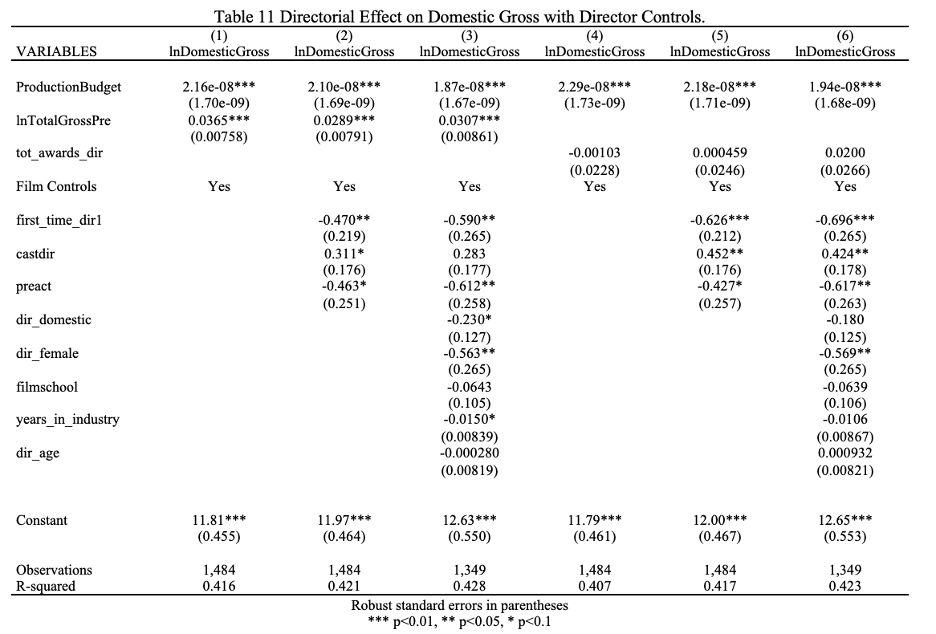
\includegraphics{./assets/thesis_table1.png}

}

\end{table}%

\begin{table}

\caption{\label{tbl-2}Directorial Effect on IMDb Rating with Director
Controls}

\centering{

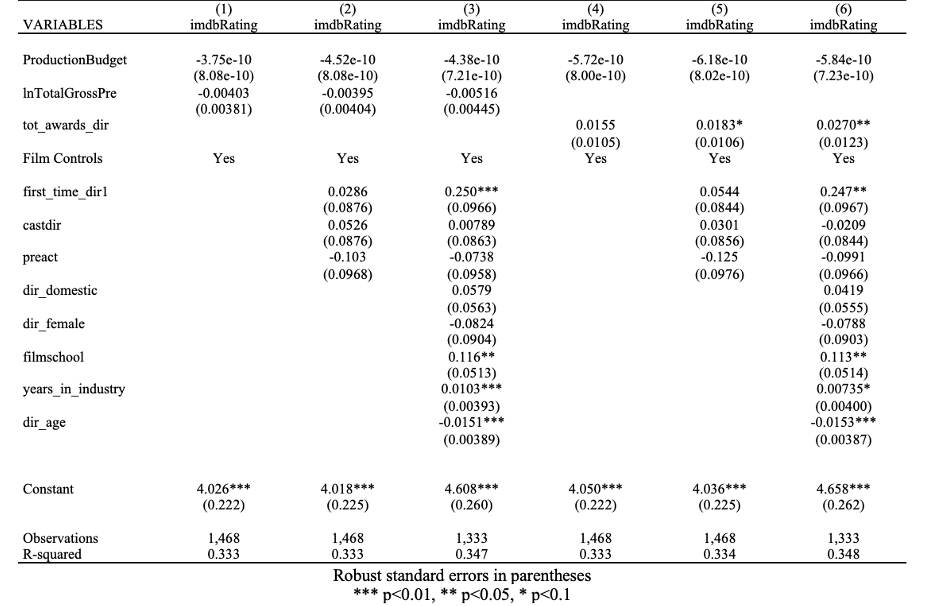
\includegraphics{./assets/thesis_table2.png}

}

\end{table}%

The paper found that an increase in director financial quality yielded
between a 0.0289\% and 0.0307\% increase in domestic gross and no impact
on IMDb rating. Conversely, director quality in terms of critical
acclaim yielded no significant impact on domestic gross, but between
0.01803 and 0.0270 point increase in IMDb rating. The paper also
discovered a statistically significant decrease in domestic gross for
female directors as compared to male directors outlined in
Table~\ref{tbl-1} and Table~\ref{tbl-2}.

Overall, the results were thought-provoking; however, the methodology
used was lacking in the causality department. The research, if anything,
worked towards establishing a weak association due to its statistical
analysis going only so far as a simple ordinary-least-squares regression
and controlling for confounding variables. While the variables were
considered and included in the regression equation, they were all
treated equally as controls; thus, a more complex analysis is warranted.

Moving forward, the work to get to causality includes introducing causal
methods for handling covariates instead of just controlling for them.
Furthermore, I wanted to investigate the conclusion of gender bias
further and shifted this analysis to examine actors instead of
directors.

Thus, this paper will investigate the impact of gender bias in the film
industry pertaining to economic outcomes. Specifically, it will attempt
to establish a causal link between a film casting a female actress in
the leading role and the resulting box-office revenue by employing
propensity score matching.

Data collection and preparation are discussed in Section~\ref{sec-data}.
Methodology, manufactured variables, and propensity scoring are
discussed in Section~\ref{sec-meth}. Results and analysis are presented
in Section~\ref{sec-results}. Results are discussed in
Section~\ref{sec-discuss}. Concluding remarks, limitations, and future
work are discussed in Section~\ref{sec-conclusion}.

\section{Data}\label{sec-data}

The data for this research was collected from two separate sources:
\href{https://www.omdbapi.com/}{Open Movie Database (OMDb)} and
\href{https://www.themoviedb.org/}{The Movie Database (TMDb)}. Both are
sources for movie and television metadata, differing only in their
sourcing and specific variables provided. OMDb partly sources from
Amazon's Internet Movie Database (IMDb) and then relies on crowdsourcing
for missing data, while TMDb is independently created and relies solely
on crowdsourcing from its community of film buffs to provide data entry
for films. Both of these sources offer an API that allowed for the
collection of movie metadata, which was then merged using an inner join
on the film Title and resulted in the following variables:
\texttt{Title}, \texttt{Year}, \texttt{Runtime}, \texttt{Budget},
\texttt{Released}, \texttt{Genre} (Action, Adventure, Animation,
Biography, Comedy, Crime, Documentary, Drama, Family, Fantasy, Film
Noir, History, Horror, Music, Musical, Mystery, Romance, Sci-Fi, Sport,
Thriller, War, Western), \texttt{MPAA\ Rating} (G, GP, M, M/PG, NC-17,
Not-Rated, PG, PG-13, R, TV-MA, Unrated, Accepted),
\texttt{Production\ Companies}, \texttt{Director}, \texttt{Writer},
\texttt{Country}, \texttt{Language}, \texttt{Description},
\texttt{Tagline}, \texttt{Overview}, \texttt{Actors},
\texttt{Box\ Office}, \texttt{Revenue}, \texttt{IMDb\ Rating},
\texttt{Metascore}, \texttt{IMDb\ Votes}, \texttt{TMDb\ rating},
\texttt{Vote\ Count}, \texttt{Awards}, and \texttt{Poster\ URL}.

With this combined dataset, some further preparation was required to
move forward with the analysis. Firstly, some variables were dropped as
they were deemed unimportant, while others were very similar across the
datasets; for example, only the `Description' was kept, and the
`Overview' variable was dropped. All missing and zero values in
numerical variables were removed, and each of the variables was
converted to the correct data type. The `Released' date was split into
three variables for the month, day, and year. For the categorical
variables, two different techniques were utilized. For `Genre' and `MPAA
rating', a one-hot encoding was applied. However, for the `Language' and
`Country' only the first observation of each was kept, which was then
categorized simply as either English or other language, and domestic
(for the US) and international for all other countries.

The final dataset included a total of 2,816 films with 61 columns of
variables.

\begin{longtable}[]{@{}lll@{}}
\caption{Summary Statistics of Numerical
Variables}\label{tbl-3}\tabularnewline
\toprule\noalign{}
Variable & Minimum & Maximum \\
\midrule\noalign{}
\endfirsthead
\toprule\noalign{}
Variable & Minimum & Maximum \\
\midrule\noalign{}
\endhead
\bottomrule\noalign{}
\endlastfoot
Box Office & 3,622 & 858,373,000 \\
Budget & 7,000 & 460,000,000 \\
Runtime & 63 & 238 \\
IMDb Rating & 1.9 & 9.3 \\
IMDb Votes & 1,672 & 3,059,994 \\
\end{longtable}

The IMDb Rating, which is a score given by the Internet Movie Database,
takes ratings given by IMDb users and aggregates them to generate a
single rating from 0 to 10 for each film, with 10 indicating a perfect
film and 0 indicating the worst possible film. In this dataset, the
lowest rating given was a 1.9, while the highest rating was a 9.3, and
the average was around a 6.6 rating. As shown in Figure~\ref{fig-2},
there is a clear decline in the average IMDb Rating over the years,
beginning around 1970 and flattening out over the last 20 or so years.

\begin{figure}

\centering{

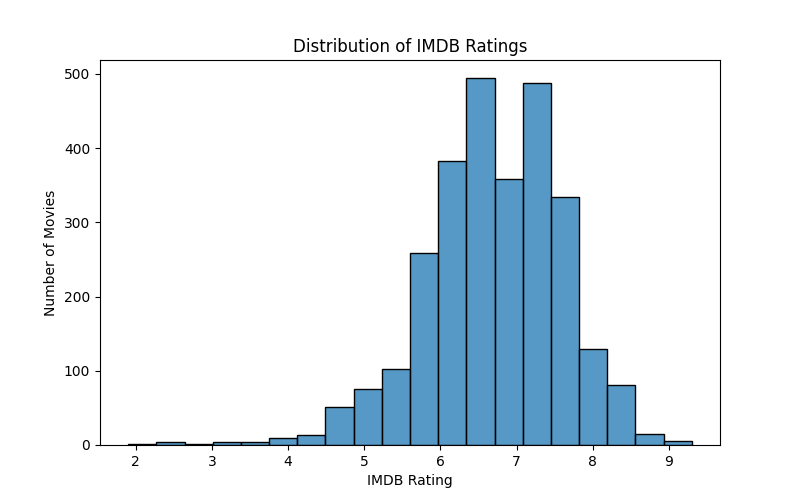
\includegraphics{./notebooks/notebook_output/imdb_rating.png}

}

\caption{\label{fig-1}IMDb Rating Distribution}

\end{figure}%

\begin{figure}

\centering{

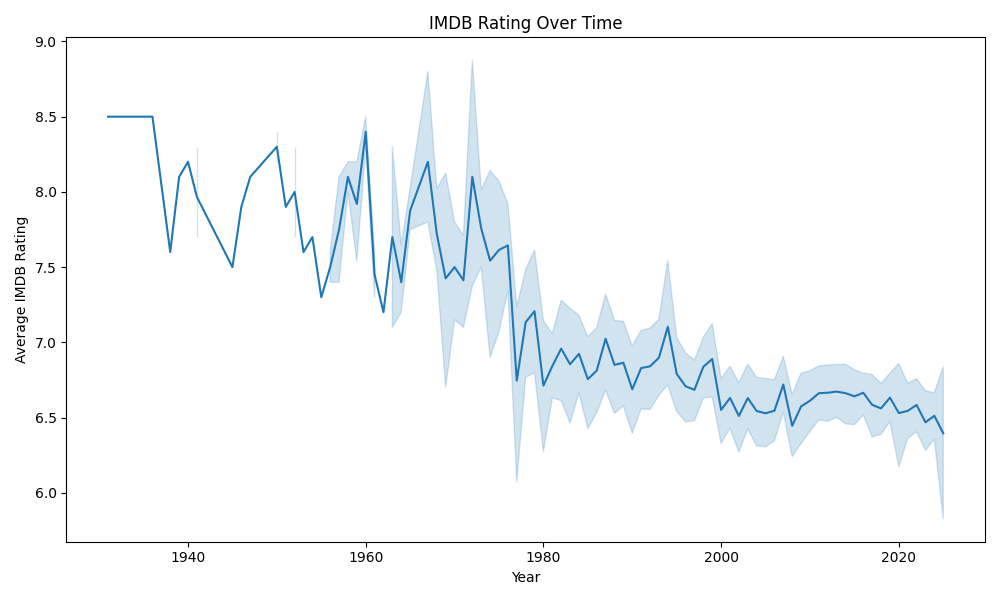
\includegraphics{./notebooks/notebook_output/imdb_overtime.png}

}

\caption{\label{fig-2}IMDb Ratings over the Years}

\end{figure}%

The Box Office value is the total revenue earned by the film from ticket
sales for the film's release in theatres only. This metric is often
utilized in entertainment economics literature as a proxy for the
success of the film. This number boosts a mean of around 73.5 million.
As shown in Figure~\ref{fig-3}, unlike the IMDb rating, the box office
has seen a general increasing trend over the years since 1970, except
for 2020 when theatres were closed due to COVID-19.

\begin{figure}

\centering{

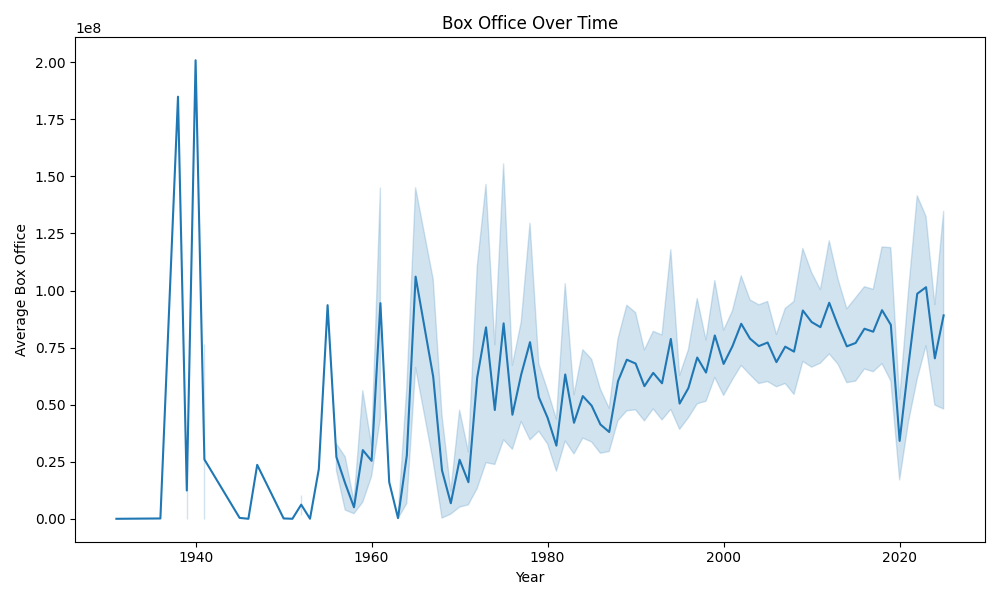
\includegraphics{./notebooks/notebook_output/boxoffice_overtime.png}

}

\caption{\label{fig-3}Box-Office Revenue over the Years}

\end{figure}%

When looking at the categorizations of the films, we see that most fall
into the genres of drama, comedy, action, and adventure and have an MPAA
rating of R, PG-13, or G (Figure~\ref{fig-4} and Figure~\ref{fig-5}).

\begin{figure}

\centering{

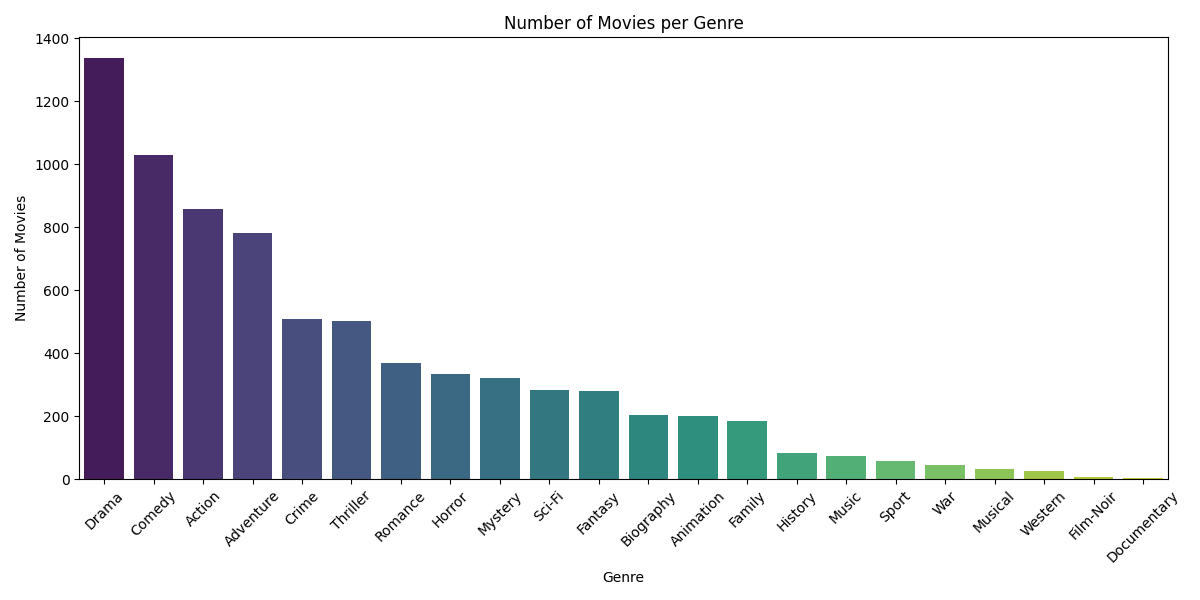
\includegraphics{./notebooks/notebook_output/genre_counts.png}

}

\caption{\label{fig-4}Distribution of Film Genres}

\end{figure}%

\begin{figure}

\centering{

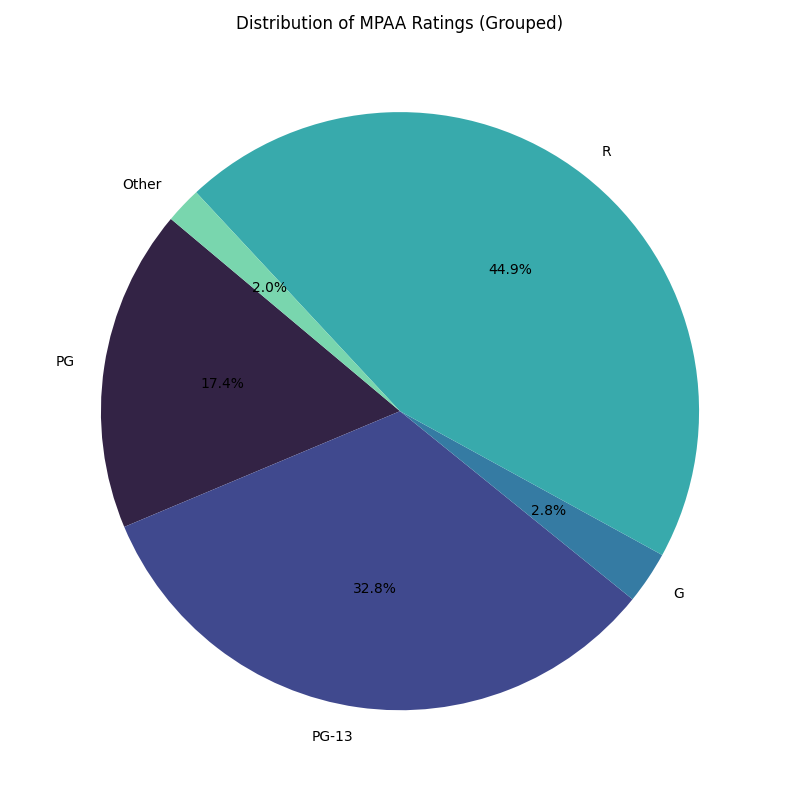
\includegraphics{./notebooks/notebook_output/mpaa_pie.png}

}

\caption{\label{fig-5}Percentage of Film MPAAs Ratings}

\end{figure}%

\section{Methodology}\label{sec-meth}

\subsection{Manufactured Variables}\label{manufactured-variables}

\subsubsection{Top Directors, Writers, Production
Companies}\label{top-directors-writers-production-companies}

In order to incorporate the level of expertise of the team creating the
film, this analysis worked to categorize the level of directors,
writers, and production companies. All of these were attempting to
better match movies based on the level of effort put into its creation
in terms of money, knowledge, experience, and previous success. To
achieve this, three lists were collected that detailed the top
directors, writers, and production companies:

{``IMDb list''} (n.d.-b)\\
{``IMDb list''} (n.d.-a)\\
{``Production companies overview''} (n.d.)

The directors and writers were judged on a combination of their
perceived skill and their lifetime achievement in terms of awards and
accolades. The production companies were compiled simply based on the
total domestic box-office revenue amassed across all films they have
produced.

The director, writer, and production company variables were then
referenced against these lists, receiving a 1 if the entity was
mentioned in the list and a 0 otherwise, resulting in three one-hot
encoded variables: \texttt{Top\_Production}, \texttt{Top\_Director}, and
\texttt{Top\_Writer}. For the sake of simplicity, if more than one
entity was listed for any of these variables, only the first entity was
taken into account.

\subsubsection{Tagline and Description Sentiment
Analysis}\label{tagline-and-description-sentiment-analysis}

In order to extract meaningful value from the film description and
tagline, sentiment analysis was performed on the text. This sentiment
analysis was performed by an off-the-shelf pre-trained model publicly
available on Hugging Face Face (n.d.) . This model was trained on
English text specifically for binary text classification and achieved a
high accuracy score. The result is two variables with a binary value of
1 for positive sentiment or 0 for negative sentiment of both the film
description and film tagline.

\begin{longtable}[]{@{}
  >{\raggedright\arraybackslash}p{(\columnwidth - 6\tabcolsep) * \real{0.3014}}
  >{\raggedright\arraybackslash}p{(\columnwidth - 6\tabcolsep) * \real{0.2877}}
  >{\raggedright\arraybackslash}p{(\columnwidth - 6\tabcolsep) * \real{0.2466}}
  >{\raggedright\arraybackslash}p{(\columnwidth - 6\tabcolsep) * \real{0.1644}}@{}}
\caption{Example of the Tagline Sentiment
Values}\label{tbl-4}\tabularnewline
\toprule\noalign{}
\begin{minipage}[b]{\linewidth}\raggedright
Title
\end{minipage} & \begin{minipage}[b]{\linewidth}\raggedright
Tagline
\end{minipage} & \begin{minipage}[b]{\linewidth}\raggedright
Tagline Sentiment
\end{minipage} & \begin{minipage}[b]{\linewidth}\raggedright
\end{minipage} \\
\midrule\noalign{}
\endfirsthead
\toprule\noalign{}
\begin{minipage}[b]{\linewidth}\raggedright
Title
\end{minipage} & \begin{minipage}[b]{\linewidth}\raggedright
Tagline
\end{minipage} & \begin{minipage}[b]{\linewidth}\raggedright
Tagline Sentiment
\end{minipage} & \begin{minipage}[b]{\linewidth}\raggedright
\end{minipage} \\
\midrule\noalign{}
\endhead
\bottomrule\noalign{}
\endlastfoot
Surf's Up & A Major Ocean Picture. & 1 & \\
The BFG & The world is more giant than you can imagine. & 1 & \\
Twin Peaks: Fire Walk with Me & In a town like Twin Peaks, no one is
innocent. & 0 & \\
Meet the Robinsons & If you think your family's different, wait 'til you
meet the family of the future. & 1 & \\
The Royal Tenenbaums & Family isn't a word \ldots{} It's a sentence. & 0
& \\
\end{longtable}

\begin{longtable}[]{@{}ll@{}}
\caption{Count of Positive and Negative
Sentiment}\label{tbl-5}\tabularnewline
\toprule\noalign{}
Sentiment & Count \\
\midrule\noalign{}
\endfirsthead
\toprule\noalign{}
Sentiment & Count \\
\midrule\noalign{}
\endhead
\bottomrule\noalign{}
\endlastfoot
Positive & 1476 \\
Negative & 1340 \\
\end{longtable}

\subsubsection{Starpower Variable}\label{starpower-variable}

One of the most important building blocks of a film is the cast of
actors and actresses, and well-known names can be a huge draw to the
theatres for movie-goers. This feature seemingly has an impact on the
outcome of the film and its financial success. Thus, finding a way to
classify the `starpowerness' of the cast was paramount to this analysis.
The dataset, unfortunately, only provides the three main cast members,
which discounts films that rely on an ensemble cast or have a large
enough budget to cast many big names. That being said, this research
attempted to define a metric that quantified this `starpower' aspect of
the three cast members, in the hopes that the success and
name-recognition can be at least partly captured.

The metric was created by collecting lists of A-list and B-list actors
and actresses.

{``IMDb a-list actors''} (n.d.)\\
{``IMDb a-list actresses''} (n.d.)\\
{``IMDb b-list actors and actresses''} (n.d.)

In film terms, these categorizations reflect how `bankable' the stars
are or how much financial draw they bring to a film, theoretically.
These lists are all collected from IMDb and include a wide range of
household names. With these lists, the cast variable was split into
\texttt{actor1}, \texttt{actor2}, and \texttt{actor3} based simply on
the order in which they were listed. Then, each of the cast variables
was referenced against all three of the lists. The film title received:

\begin{itemize}
\tightlist
\item
  \textbf{2 points} if a cast member was part of the A-list\\
\item
  \textbf{1 point} if a cast member was part of the B-list
\end{itemize}

These points were added in the \texttt{starpower} variable and then
divided by three to get a finalized score of the points across the three
cast members. Table~\ref{tbl-6} shows an example of the scoring.

\begin{longtable}[]{@{}
  >{\raggedright\arraybackslash}p{(\columnwidth - 6\tabcolsep) * \real{0.3014}}
  >{\raggedright\arraybackslash}p{(\columnwidth - 6\tabcolsep) * \real{0.2877}}
  >{\raggedright\arraybackslash}p{(\columnwidth - 6\tabcolsep) * \real{0.2466}}
  >{\raggedright\arraybackslash}p{(\columnwidth - 6\tabcolsep) * \real{0.1644}}@{}}
\caption{Starpower Metric Scores for the Cast of 10
Films}\label{tbl-6}\tabularnewline
\toprule\noalign{}
\begin{minipage}[b]{\linewidth}\raggedright
actor1
\end{minipage} & \begin{minipage}[b]{\linewidth}\raggedright
actor2
\end{minipage} & \begin{minipage}[b]{\linewidth}\raggedright
actor3
\end{minipage} & \begin{minipage}[b]{\linewidth}\raggedright
starpower
\end{minipage} \\
\midrule\noalign{}
\endfirsthead
\toprule\noalign{}
\begin{minipage}[b]{\linewidth}\raggedright
actor1
\end{minipage} & \begin{minipage}[b]{\linewidth}\raggedright
actor2
\end{minipage} & \begin{minipage}[b]{\linewidth}\raggedright
actor3
\end{minipage} & \begin{minipage}[b]{\linewidth}\raggedright
starpower
\end{minipage} \\
\midrule\noalign{}
\endhead
\bottomrule\noalign{}
\endlastfoot
Mark Wahlberg & Tyrese Gibson & André 3000 & 0.666667 \\
Jamie Bell & Andy Serkis & Daniel Craig & 1.333333 \\
Ryan Reynolds & Blake Lively & Peter Sarsgaard & 0.333333 \\
Marc Singer & Tanya Roberts & Rip Torn & 0.000000 \\
Tom Hiddleston & Samuel L. Jackson & Brie Larson & 1.000000 \\
Jeremy Renner & Ed Helms & Jake Johnson & 0.000000 \\
Frankie Muniz & Amanda Bynes & Paul Giamatti & 1.000000 \\
Ben Barnes & Skandar Keynes & Georgie Henley & 0.000000 \\
Jason Bateman & Charlie Day & Jason Sudeikis & 1.000000 \\
Jack Black & Ana de la Reguera & Héctor Jiménez & 0.333333 \\
\end{longtable}

\subsubsection{Feamle Leading Role
Variable}\label{feamle-leading-role-variable}

This analysis relied on the ability to distinguish between female and
male leading actresses and actors; however, this is not something
directly encoded into the metadata of a film, thus this variable had to
be manufactured. In order to achieve this, a list of all current female
actresses was collected from Wikipedia {``List of american film
actresses''} (n.d.). This list included 2,816 names of female actresses,
alphabetized. To note, there were attempts to utilize a list of all
female names and an off-the-shelf model to guess whether the cast member
listed identified as male or female, however, both of these methods
produced more inaccuracy, thus the list of female actresses method was
proceeded with.

The next step was to determine only the presumed lead cast member by
extracting the first person listed in the \texttt{actors} variable of
the dataset. This name was then compared against the list of female
actresses and received a value of 1 if the cast member was included on
the list.

Therefore, the result was a variable titled \texttt{female\_lead} if the
first cast member listed in the IMDb metadata was a member of the
current working female actress list and a 0 if the cast member was not a
member of the list and, thus, presumably a male actor. Table~\ref{tbl-7}
displays an example of the accuracy results of this variable.

\begin{longtable}[]{@{}lll@{}}
\caption{Example of the \texttt{female\_lead}
Variable}\label{tbl-7}\tabularnewline
\toprule\noalign{}
Title & First Actor & Female Lead \\
\midrule\noalign{}
\endfirsthead
\toprule\noalign{}
Title & First Actor & Female Lead \\
\midrule\noalign{}
\endhead
\bottomrule\noalign{}
\endlastfoot
The Family & Robert De Niro & 0 \\
The Shack & Sam Worthington & 0 \\
The Dead Zone & Christopher Walken & 0 \\
The Ref & Denis Leary & 0 \\
Flyboys & James Franco & 0 \\
ATL & Tip `T.I.' Harris & 0 \\
Like a Boss & Tiffany Haddish & 1 \\
Enemy Mine & Dennis Quaid & 0 \\
Proud Mary & Taraji P. Henson & 1 \\
Valmont & Colin Firth & 0 \\
\end{longtable}

As displayed in Table~\ref{tbl-8} the films were split between 488 films
with female leading actresses and 2328 films with male leading actors.

\begin{longtable}[]{@{}ll@{}}
\caption{Male Versus Female Director Counts}\label{tbl-8}\tabularnewline
\toprule\noalign{}
Name & Year \\
\midrule\noalign{}
\endfirsthead
\toprule\noalign{}
Name & Year \\
\midrule\noalign{}
\endhead
\bottomrule\noalign{}
\endlastfoot
Female Leads & 488 \\
Male Leads & 2328 \\
\end{longtable}

\subsection{Propensity Score Matching}\label{propensity-score-matching}

With these manufactured variables created, the primary statistical
analysis performed was propensity score matching (PSM). This statistical
method allows for comparison of films that are similar across all
observed covariates, differing only in whether the lead is a male or
female actor or actress. In this context, the presence of a female lead
is handled as a treatment, and the effect of that treatment on the
outcome variable is estimated.

Unlike simply including covariates as controls in a regression equation,
this technique aims to reduce selection bias by matching treated and
control units based on their likelihood of receiving the treatment,
given the covariates. This creates a more comparable dataset, which
quasi-mimics the conditions of a randomized experiment.

The process of propensity score matching began with normalizing the
variables due to the very differing range of values across variables
like the IMDb rating (which is 0-10) and the budget (which can reach
hundreds of millions). This was done with Sklearn's StandardScaler
scikit-learn developers (2025) and performed on all numerical variables.

Following this step, the variance inflation factor (VIF) was checked to
investigate any multicollinearity issues among the covariates that would
bias the analysis. This yielded some problematic variables, which
resulted in excluding those that exceeded the VIF threshold of 10
points. The following variables were excluded: international country
(domestic country kept), other language (English kept), musical genre
(all other genre categories kept), and accepted MPAA rating (all other
MPAA ratings kept).

Next, a logistic regression was estimated. The variables
\texttt{metascore}, \texttt{IMDb\ votes}, \texttt{TMDb\ rating},
\texttt{TMDb\ votes}, \texttt{Oscars\ Won}, \texttt{Oscars\ Nominated},
\texttt{Award\ Wins}, and \texttt{Award\ Nominations} were omitted
because they are ex-post variables, meaning they represent effects of
the outcomes as opposed to causes of it, thus creating data leakage and
bias. Therefore, only ex-ante variables are considered. The resulting
equation is as follows, representing a female leading role as the
treatment and the film characteristics as covariates:

\begin{align}
\text{logit}(\mathbb{P}(\text{Female\_Lead} = 1)) &= \beta_0 
+ \beta_1 \cdot \text{Year}
+ \beta_2 \cdot \text{Runtime}
+ \beta_3 \cdot \text{Budget}
+ \beta_4 \cdot \text{Month}
+ \beta_5 \cdot \text{Day} \nonumber \\
&\quad + \sum_{g} \beta_g \cdot \text{Genre}_g
+ \sum_{r} \beta_r \cdot \text{Rating}_r \nonumber \\
&\quad + \beta_6 \cdot \text{Top\_Production\_Company}
+ \beta_7 \cdot \text{Top\_Director}
+ \beta_8 \cdot \text{Top\_Writer} \nonumber \\
&\quad + \beta_9 \cdot \text{Domestic}
+ \beta_{10} \cdot \text{English\_Language} \nonumber \\
&\quad + \beta_{11} \cdot \text{Descr\_Sentiment}
+ \beta_{12} \cdot \text{Tagline\_Sentiment}
+ \beta_{13} \cdot \text{Starpower}
\end{align}

The result of this equation is propensity scores (ps) for each film
title (dataset row), which represent the calculated probability of the
film having a female leading actress. A score close to 0 indicates a
higher likelihood of the film having a male lead, while a score closer
to 1 indicates a higher likelihood of a film having a female lead. These
scores are then used to match, utilizing 1:1 nearest neighbor matching,
the movies across the two groups of leading actors/actresses based on
the closest propensity score. This results in a matched dataset with
each row being a matched pair of films that are similar in all aspects
except for the leading role.

\begin{longtable}[]{@{}lll@{}}
\caption{Example of Propensity Score Matching Between Male and Female
Led Films}\label{tbl-9}\tabularnewline
\toprule\noalign{}
Female Led Movie & PS Female & Male Led Movie \\
\midrule\noalign{}
\endfirsthead
\toprule\noalign{}
Female Led Movie & PS Female & Male Led Movie \\
\midrule\noalign{}
\endhead
\bottomrule\noalign{}
\endlastfoot
Miss Congeniality & 0.082866 & Back to the Future Part III \\
GI Jane & 0.031775 & Gladiator \\
Freaky Friday & 0.212226 & The Boat the Rocked \\
Kill Bill: Vol. 2 & 0.066924 & 2 Fast 2 Furious \\
\end{longtable}

The final step was to calculate and compare the box-office performance
of matched female versus male lead films. These results are discussed in
Section~\ref{sec-results}.

\subsection{Robustness Checks}\label{robustness-checks}

As a robustness check, the \texttt{IMDb\ rating}, which is a score from
0-10, calculated from a weighted average of user ratings on the Internet
Movie Database, is utilized as a secondary outcome variable. The same
methodology of propensity score matching is used; however, the analysis
now investigates whether a female lead role causes a change in the
critical success of the film.

\section{Results}\label{sec-results}

\begin{longtable}[]{@{}lll@{}}
\caption{Mean of Box Office and IMDb Rating for Male Versus Female Led
Films}\label{tbl-10}\tabularnewline
\toprule\noalign{}
Gender of Lead Role & Box Office & IMDb Rating \\
\midrule\noalign{}
\endfirsthead
\toprule\noalign{}
Gender of Lead Role & Box Office & IMDb Rating \\
\midrule\noalign{}
\endhead
\bottomrule\noalign{}
\endlastfoot
Female & 62,708,871.36 & 6.329 \\
Male & 61,076,707.45 & 6.601 \\
\end{longtable}

\subsection{Box Office}\label{box-office}

As shown in Table~\ref{tbl-10}, the initial hypothesis of this research
that films featuring a woman in the leading role would generate lower
box-office revenues was not supported by the analysis. In fact, the
opposite was found: that female films earned an average of \$62,708,871,
while male films earned an average of \$61,076,707 in box-office
revenues. This means that female-led films earned 1,632,163.91 more at
the box office on average. While the magnitude of the difference is
modest compared to the average box-office revenue, the matched sample
analysis does suggest that having a female lead was associated with
slightly higher box-office performance.

\subsection{IMDb Rating}\label{imdb-rating}

The robustness check, which substituted IMDb rating as the outcome
variable (also in Table~\ref{tbl-10}), revealed a different pattern.
Female-led films had an average IMDb rating of 6.329, while male-led
films had an average of 6.601, a difference of -0.272. This indicated
that, on average, female-led films received a 0.272 lower audience
rating than male-led films despite their slightly better box-office
results.

\section{Discussion}\label{sec-discuss}

There are a couple of plausible explanations for the disparity of these
results. As one explanation, this could be an indication that the
general public of individuals who partake in film going casually have
fully accepted female-led films and even enjoy them more. However, film
critics and individuals who view films more seriously are less accepting
of women playing large roles in films. Another explanation is that women
are cast in roles that seemingly lack depth and thus are less likely to
receive critical success, meaning filmmakers are combining women leading
roles with less serious script material, but still casting them in
blockbuster films that draw an audience. Furthermore, this could
indicate an audience leaning toward certain female actresses or female
actresses in general, pushing box-office numbers higher.

The analysis, while offering insightful results, still faced some
limitations. Firstly, there is always room for more data and a larger,
more encompassing dataset. With a little over 2,000 films, the dataset
barely scratches the surface of the total filmography possible, and more
data would allow for more accurate propensity score matching. Secondly,
the `starpower' metric is quite subjective in that the lists of
A-listers and B-listers were based on opinions about the actors and
actresses, instead of some numeric metric. Thirdly, there is a small
level of inaccuracy with the creation of the female lead variable. While
the list of actresses utilized was quite large, it was not fully
encompassing; thus, some actresses were not classified correctly.
Furthermore, this variable was created solely by splitting the cast list
and taking the first name, which is not necessarily the lead cast member
in all cases, and disregards films that have more than one leading actor
or actress or have an ensemble cast.

These limitations offer much room for future work. To start, a more
detailed and objective metric of the `starpower' variable could be
useful, as this is a huge determinant of the making of a film. This
could be performed with network analysis of the cast to determine the
centrality of the actors as a measure of their importance in the
industry. In addition, classifying the tagline and description based on
content instead of sentiment could add more depth to the propensity
scoring. Similarly, a more comprehensive look at the film genres could
create better matches. This could be done by leveraging an LLM to score
the film from 0-1 for each genre, indicating how much the film falls
into that category, instead of weighting each genre listed equally.
Finally, implementing a different gender-based treatment variable could
be a telling robustness check. For example, defining the treatment as
films that pass the Bechdel test could create a more accurate look at
how gender roles truly impact the outcome of the film.

\section{Conclusion}\label{sec-conclusion}

Taken together, the findings offer opposing views of how gender matters
in the film industry. The box office analysis suggests a positive causal
relationship between a female in the title role and revenue performance,
while the IMDb rating analysis suggests a negative causal relationship
between female leads and audience ratings.

Whatever the underlying reasoning, the differing results underscore the
complexity of the relationship between gender representation in leading
roles and measures of film success. This highlights the importance of
considering multiple outcome variables when assessing potential
treatment effects, especially when dealing with a topic as nuanced as
film and entertainment.

\section*{References}\label{references}
\addcontentsline{toc}{section}{References}

\vspace{1em}

\textsubscript{Source:
\href{https://ehealy19.github.io/Matching_Movies/index.qmd.html}{Article
Notebook}}

\phantomsection\label{refs}
\begin{CSLReferences}{1}{0}
\bibitem[\citeproctext]{ref-distilbert_sst2_hf}
Face, H. (n.d.n.d.). Distilbert-base-uncased-finetuned-sst-2-english.
\url{https://huggingface.co/distilbert/distilbert-base-uncased-finetuned-sst-2-english}.

\bibitem[\citeproctext]{ref-imdb_a_list_actors}
IMDb a-list actors. (n.d.).
\url{https://www.imdb.com/list/ls056262001/}.

\bibitem[\citeproctext]{ref-imdb_a_list_actresses}
IMDb a-list actresses. (n.d.).
\url{https://www.imdb.com/list/ls056262192/}.

\bibitem[\citeproctext]{ref-imdb_b_list}
IMDb b-list actors and actresses. (n.d.).
\url{https://www.imdb.com/list/ls024783564/}.

\bibitem[\citeproctext]{ref-imdb_top_writers}
IMDb list: Top 20 greatest screenwriters of all time. (n.d.-a).
\url{https://www.imdb.com/list/ls064457317/}.

\bibitem[\citeproctext]{ref-imdb_top_directors}
IMDb list: Top 25 greatest directors of all time. (n.d.-b).
\url{https://www.imdb.com/list/ls052380992/}.

\bibitem[\citeproctext]{ref-wiki_film_actresses}
List of american film actresses. (n.d.).
\url{https://en.wikipedia.org/wiki/List_of_American_film_actresses}.

\bibitem[\citeproctext]{ref-science_cinema_history}
National Science and Media Museum. (2020). A very short history of
cinema.
\url{https://www.scienceandmediamuseum.org.uk/objects-and-stories/very-short-history-of-cinema}.

\bibitem[\citeproctext]{ref-the_numbers_production_companies}
Production companies overview. (n.d.).
\url{https://www.the-numbers.com/movies/production-companies/\#production_companies_overview=od1}.

\bibitem[\citeproctext]{ref-scikit_learn_standardscaler}
scikit-learn developers. (2025). StandardScaler --- scikit-learn 1.7.1
documentation.
\url{https://scikit-learn.org/stable/modules/generated/sklearn.preprocessing.StandardScaler.html}.

\bibitem[\citeproctext]{ref-statista_film}
Statista. (n.d.n.d.). Film production worldwide - statista topic
overview.
\url{https://www.statista.com/topics/5431/film-production-worldwide/}.

\end{CSLReferences}




\end{document}
